\documentclass[a4paper]{article}

%% Language and font encodings
\usepackage[english]{babel}
\usepackage[utf8x]{inputenc}
\usepackage[T1]{fontenc}

%% Sets page size and margins
\usepackage[a4paper,top=2.5cm,bottom=2.5cm,left=2.5cm,right=2.5cm,marginparwidth=1.75cm]{geometry}

%% Useful packages
\usepackage{amsmath}
\usepackage{graphicx}
\usepackage[colorinlistoftodos]{todonotes}
\usepackage[colorlinks=true, allcolors=blue]{hyperref}
\usepackage{subfigure}
\usepackage{caption}
\usepackage{amsfonts}
\usepackage{amsthm}
\usepackage{upquote}
\usepackage{listings}
\usepackage{enumitem}
\usepackage{dirtytalk}
\usepackage{hyperref}
\usepackage{float}

\usepackage{xcolor}
\usepackage{indentfirst}

\linespread{1.1}

\definecolor{mGreen}{rgb}{0,0.6,0}
\definecolor{mGray}{rgb}{0.5,0.5,0.5}
\definecolor{mPurple}{rgb}{0.58,0,0.82}
\definecolor{backgroundColour}{rgb}{0.95,0.95,0.92}
\lstdefinestyle{CStyle}{
    backgroundcolor=\color{backgroundColour},
    commentstyle=\color{mGreen},
    keywordstyle=\color{magenta},
    numberstyle=\tiny\color{mGray},
    stringstyle=\color{mPurple},
    basicstyle=\footnotesize,
    breakatwhitespace=false,
    breaklines=true,
    captionpos=b,
    keepspaces=true,
    numbers=left,
    numbersep=5pt,
    showspaces=false,
    showstringspaces=false,
    showtabs=false,
    tabsize=2,
    language=C
}


\def\therefore{\boldsymbol{\text{ }
\leavevmode
\lower0.4ex\hbox{$\cdot$}
\kern-.5em\raise0.7ex\hbox{$\cdot$}
\kern-0.55em\lower0.4ex\hbox{$\cdot$}
\thinspace\text{ }}}

\title{A Journey to the Interactive 3D Fractal World}
\author{CSED Yang Junha 20160785, Ryu Sangwoo 20160845, Sung Haebin 20160463}

\begin{document}
\maketitle
\begin{abstract}

\end{abstract}
\section{Motivation}

\section{Theoretical Backgrounds}
\subsection{Fractal}
\subsection{Mandelbrot Set}

\section{Task}
\subsection{Overall Structure}
\subsection{Tasks}


\section{Ideas and Implmentation}
\subsection{Development Enviornment and Codes}
We develop everything in C++ and OpenGL only.
As we mentioned in proposal, utilizing shaders directly is essential for what we do.
Thus we chose OpenGL for our development environment.

If you want to know about details about our codes,
we recommend you to read Assignment 2-4 report of Yang and Sung, because we adopt basic OpenGL structure from those.
Here are some notable source codes.
\begin{itemize}
  \item void CGraphics::M\_SimplePolyFractal(void) constructs hierarchy for fractal.
  \item void CGraphics::M\_RenderFractal(void) renders fractal.
  \item bool CGraphics::M\_MoveRequest(Vec3d d) takes movement info and expands. (see \ref{sssec:num1}.)
  \item `ver\_shd.glsl' and `frag\_test.glsl' are shaders for fractal.
\end{itemize}
\subsection{Rendering a Mandelbrot set}

\begin{lstlisting}[style=CStyle]
int main(void)
{
  printf("If you want to paste code here then do this way");
}
\end{lstlisting}
\subsection{3D Geometric Fractals}
\subsubsection{Meshes}
We have two basic meshs to implement geometric fractals. One is sphere with 6 holes, another is wormhole to connect between spheres. Because we have to connect to meshes smoothly, we construct wormhole with splines covering sphere using Loft NURBS in MAXON Cinema 4D, and apply subdivision surface.

Mesh with one sphere and one wormhole is one node in hierachical structure, and basic unit of expansion.
\begin{figure}[H]
\centering
\subfigure[Sphere with 6 holes]
{
    \label{fig:subfig1}
    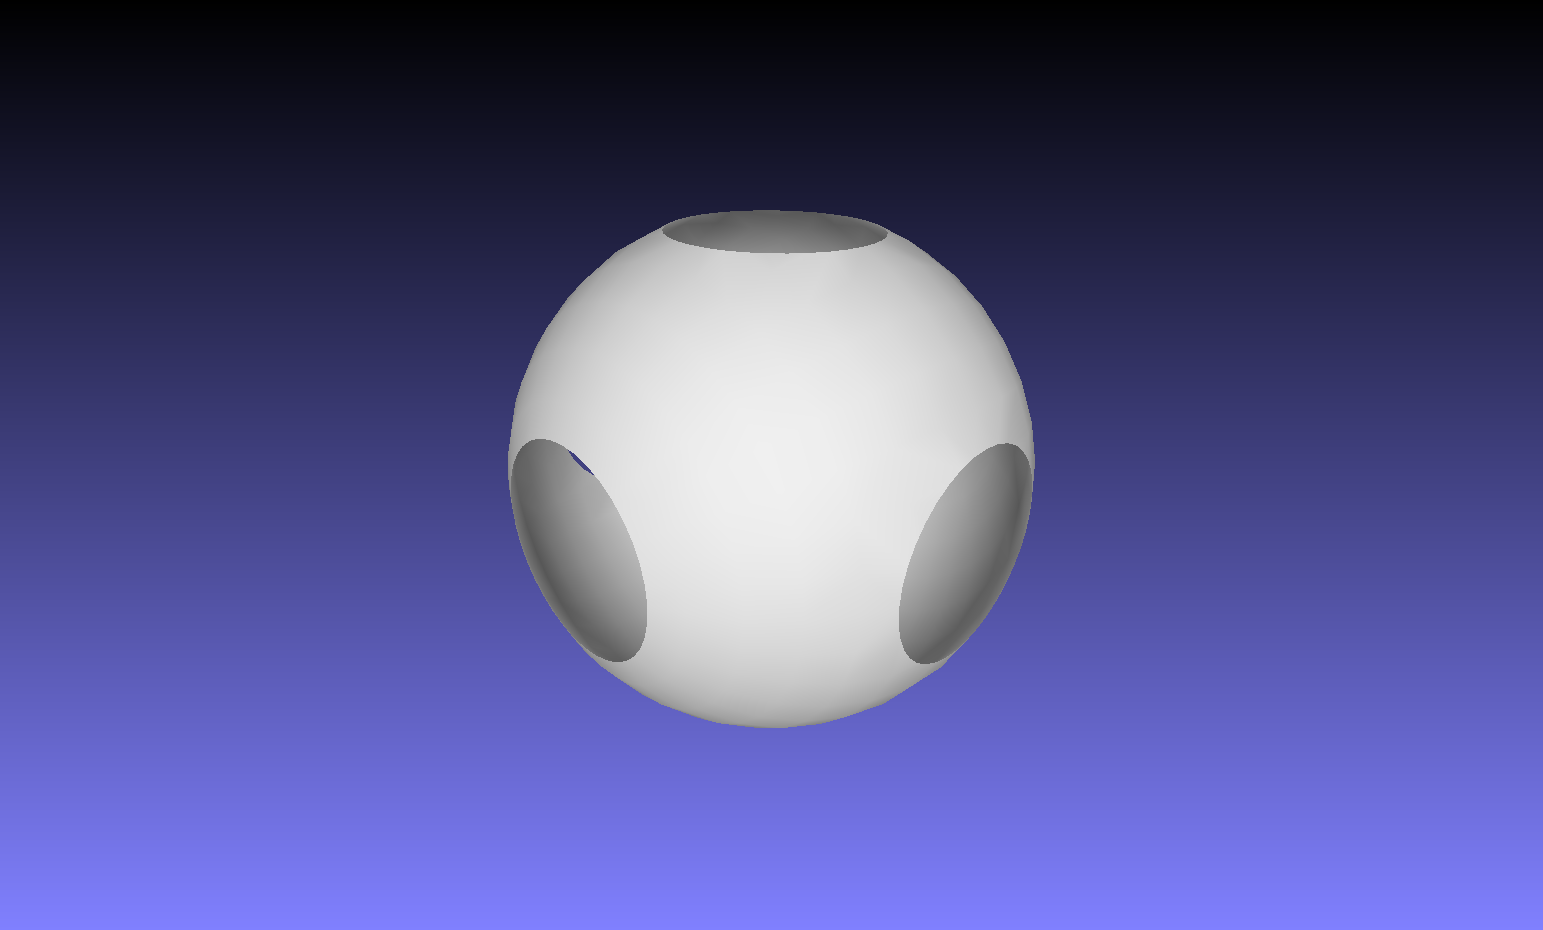
\includegraphics[scale=0.1]{sphere.png}
}
\subfigure[Wormhole]
{
    \label{fig:subfig1}
    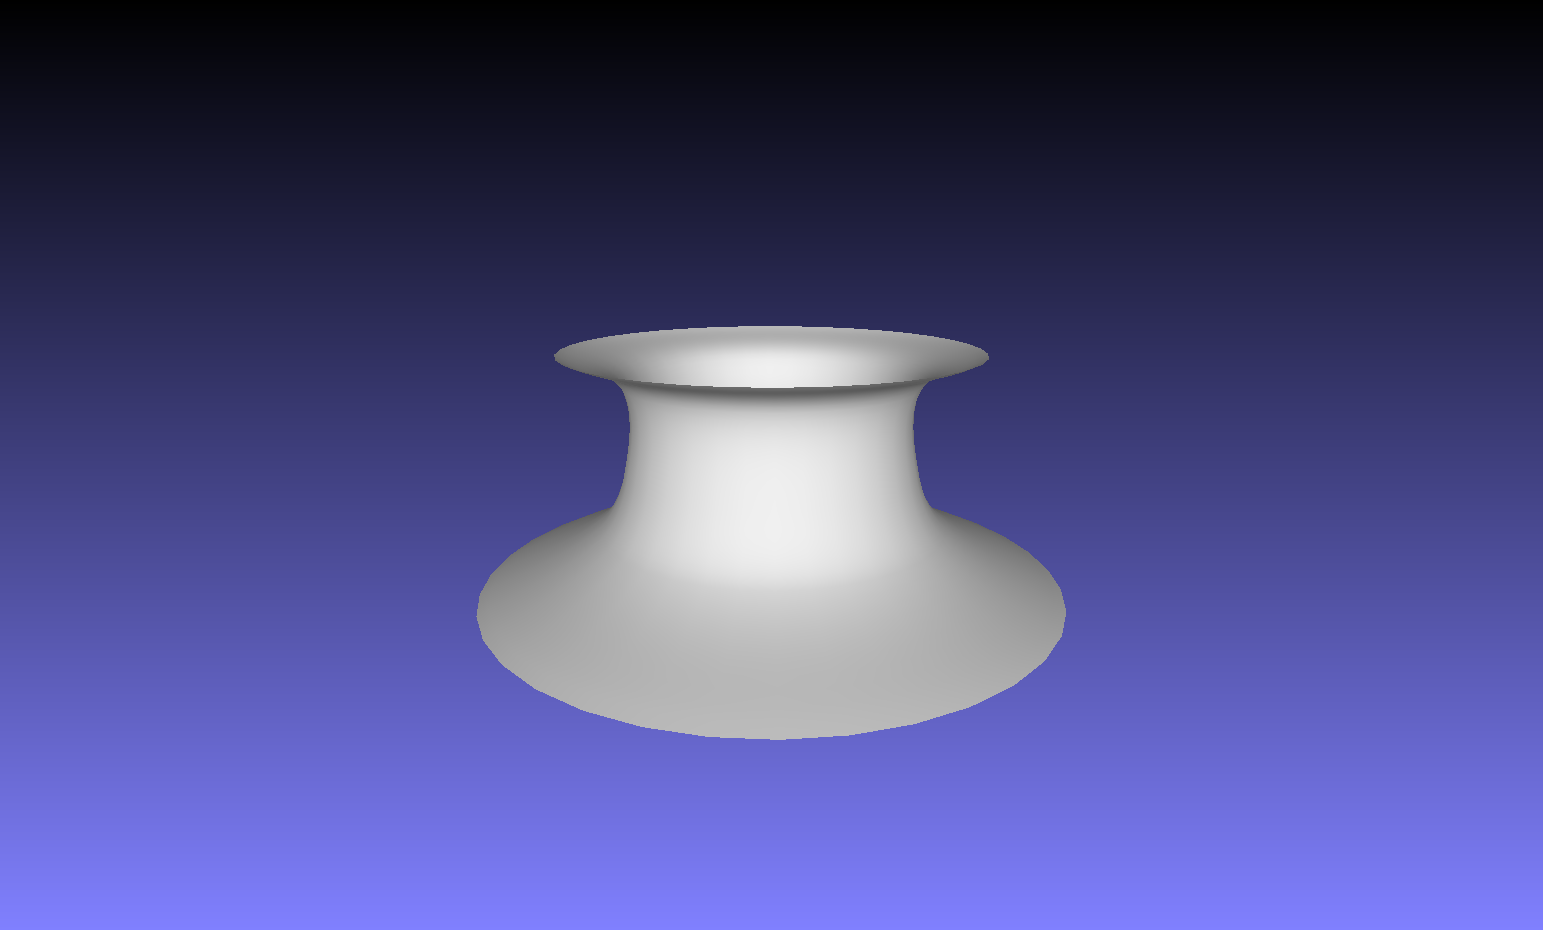
\includegraphics[scale=0.1]{wormhole.png}
}
\caption[1]{Hierarchical model for fractal.}
\end{figure}

\subsubsection{Hiearchy}
Geometric fractals can be regarded as a special case of \textit{hierarchical model}.
But, the hierarchical transfomrations are given \textit{recursively}, and each nodes have same rendering function.
If we give two recursive hierarchical transfomrations, then the fractal will grow double for each step, because the tree will be branched twice.
Then specify the maximum depth, and we can get a nice geometric fractal.
In this project, we construct the geometric fractal with 5 recursive transformation.
\begin{figure}[H]
\centering
\subfigure[5 direction of recursive transformations]
{
    \label{fig:subfig1}
    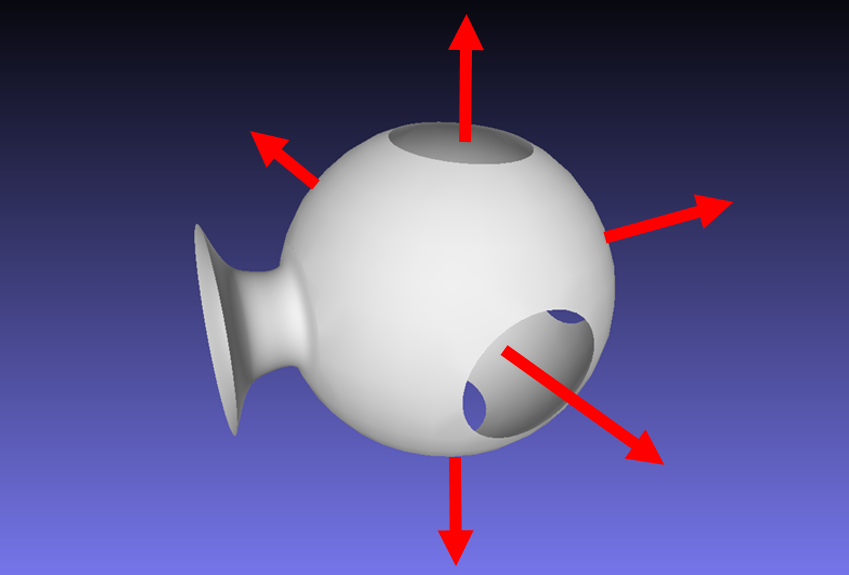
\includegraphics[scale=0.2]{hier.PNG}
}
\subfigure[Exapnded in maximum steps of 2]
{
    \label{fig:subfig1}
    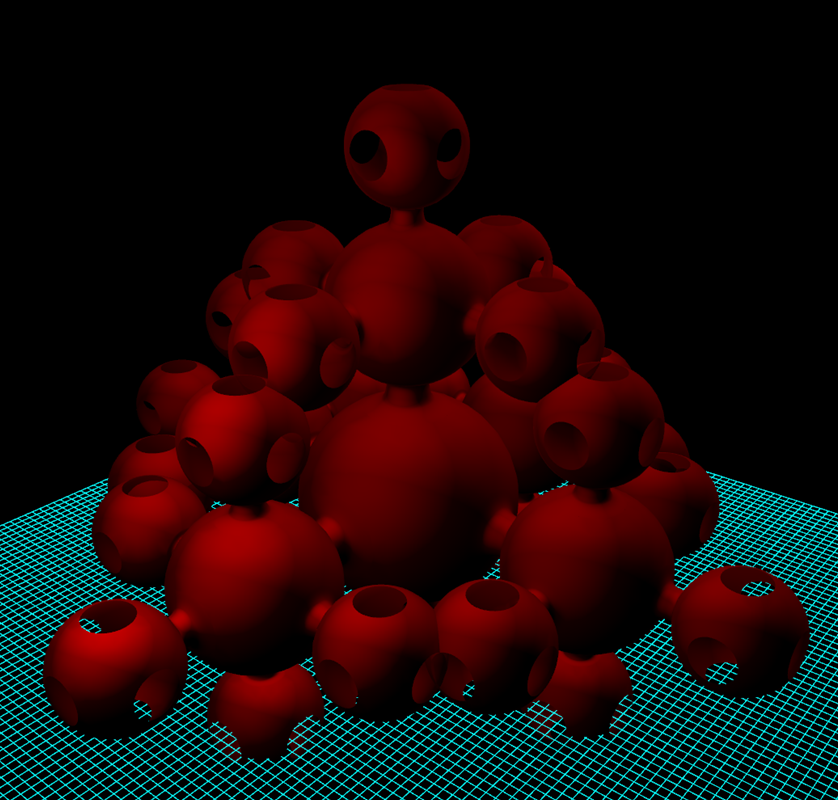
\includegraphics[scale=0.2]{expand.PNG}
}
\caption[1]{Hierarchical model for fractal.}
\end{figure}

\subsubsection{Path Tracking}\label{sssec:num1}
To `wander' into the fractal world, that geometric fractal should be somewhat `surrounding' environment for viewer.
That means the camera will move \textit{inside} the fractal, and the should able to explore deeply.
This going-through must be availiable infinitely, and this is a problem.

If we simply expand fractal in more depth, the program will die soon. (remember that the nodes grow exponentially.)
Even 10 steps require $5^{10}=9,765,6254$ nodes in the scene.
Thus we should render only relevant nodes according to current position of camera.
The idea here is to keep track of recursion path of current node.

\begin{figure}[H]
\centering
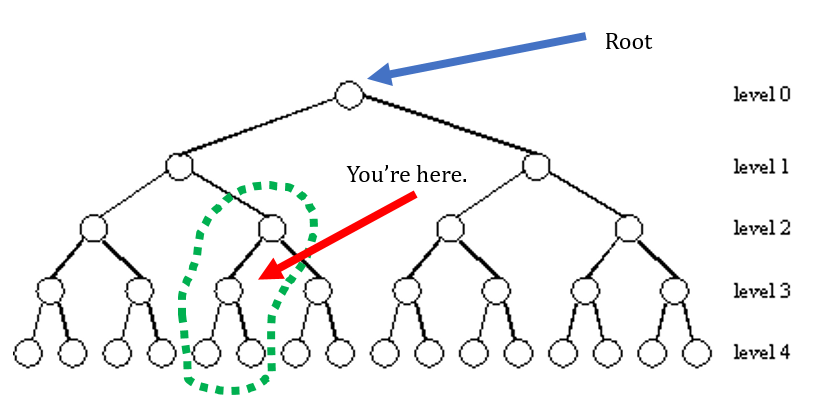
\includegraphics[scale=0.5]{tree.png}
\caption[q]{Recursive hierarchy tree. Note that the branches are reduced in 2 steps for simplicity.}
\label{fig:tree}
\end{figure}

If the program keep track of the path which the camera had moved along, then we know exactly where we are in big tree of hierarchy.
Then, the rendering pipeline can choose \textit{relevant} nodes to camera, and can partially render them.
For example, in \ref{marker}, those nodes in the green line will be chosen to be rendered.

To track the path(or trace), we should check every single movement of camera.
If the camera goes outside of current node, then see the direction(one of 5) and push it on path stack.
\begin{enumerate}
  \item Accumulate all recursive transformation using the path.
  \item Get the transformation M.
  \item Take inverse of M and multiply on my position to take everything into node(model) space.
  \item Perform a collision detection for each 6 sides of node.
  \item Find out the branch of recursion and stack on my path.
\end{enumerate}


\subsection{Texture Mapping}
Now we have to combine those seemingly independent two fractals (Mandelbrot and geometric).
Again, our approach is `fractal on fractal' and key idea is take Mandelbrot set as a `texture' for the polygons, the geometric fractal.



\subsection{Shading}
Shading is important for viewer to percept spatial structure even in non realistic fractal world.
It could be confusing to wander 6-sided chambers freely in 3D dimension.
So we applied basic shading (diffuse, specular ...) on polygons.
Assignment4 was helpful for this.

\subsection{Deformations}

\subsection{Camera control}
We have two methods moving camera. One is with keyborad input, another is with mouse moving. When we give keyboard input, camera moves to 6 direction without rotation. When we give mouse moving, camera rotates. To implement advanced camera, that is, to implement smooth movement when we give input, we introduced time variation to movement.
\begin{itemize}
  \item void CGraphics::M\_MoveCamera(void) moves camera with smooth motion.
\end{itemize}

In case of keyboard, we just give acceleration when camera starts and stops moving. In case of mouse, we interpolated mouse position with logarithmic term that depends on time.

\subsection{Antialiasing}
Antialiasing is one of the important process in high-quality rendering.
For the geometric fractal, only multi-sampling is ok because it consists of just polygons.
However the textured Mandelbrot set can't be antialiased in that way because it shows very complex structrue in \textit{pixel level}.
Of course all pixel-level rendering doesn't have to be antialiased.
For example, antialiasing the shading won't that helpful because it is inherently smooth.
But Mandelbrot set is very complicatedly structured and the pixels vary greatly, so antialisaing maybe essential.

Unfortunately, we concluded that the only way to perform antialiasing is by super-sampling because there's no way to infer something, but only calculating multiple times.
Thus we tried to perform antialiasing in fragment shader by doing Mandelbrot set membership test multiple times.
We varies testing coordinates slightly within an one pixel size for each sampling, and blend them for final output.

\begin{figure}[H]
\centering
\subfigure[Mandelbrot set without antialiasing]
{
    \label{fig:subfig1}
    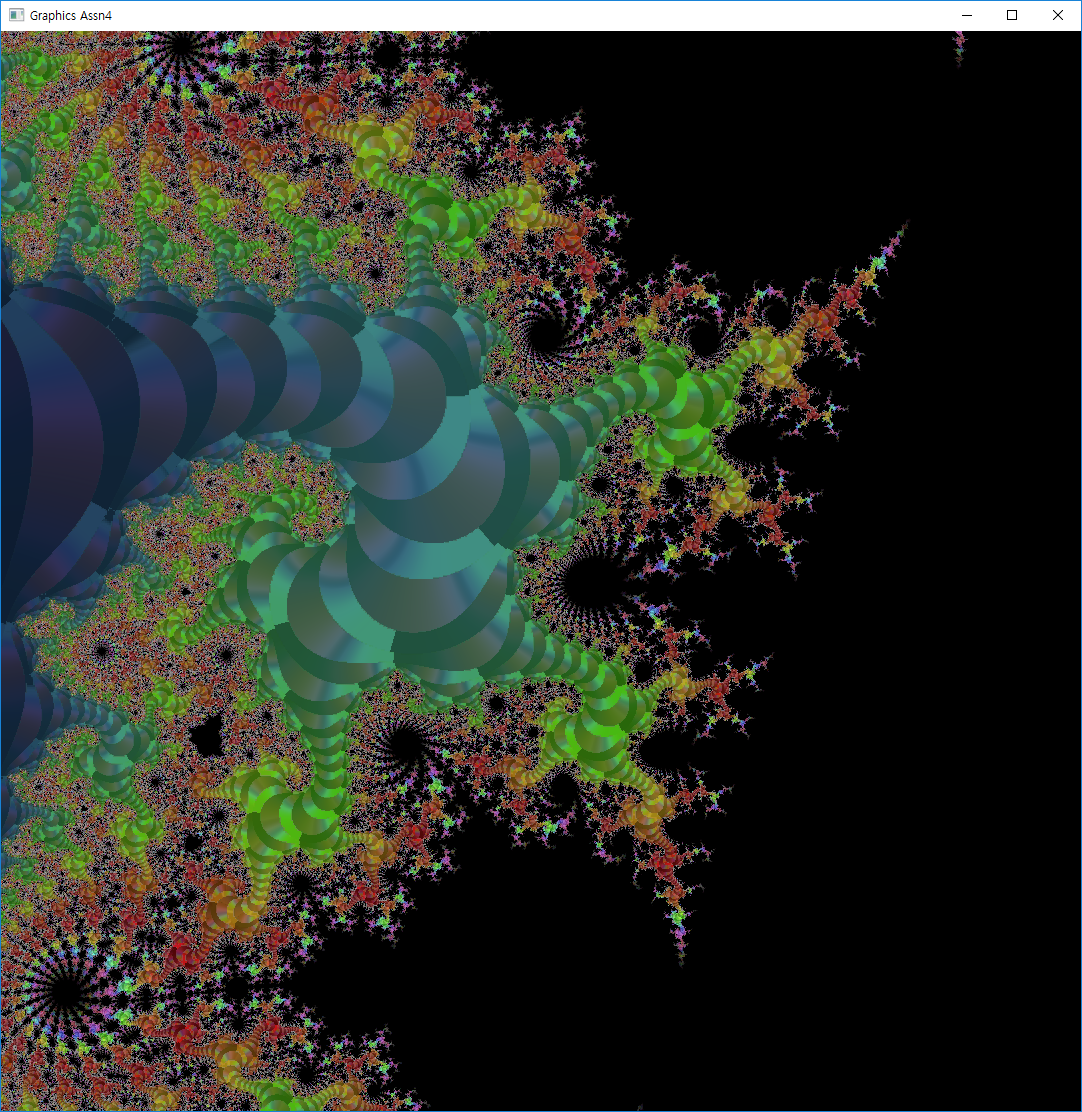
\includegraphics[scale=0.2]{noanti.PNG}
}
\subfigure[Mandelbrot set with antialiasing]
{
    \label{fig:subfig1}
    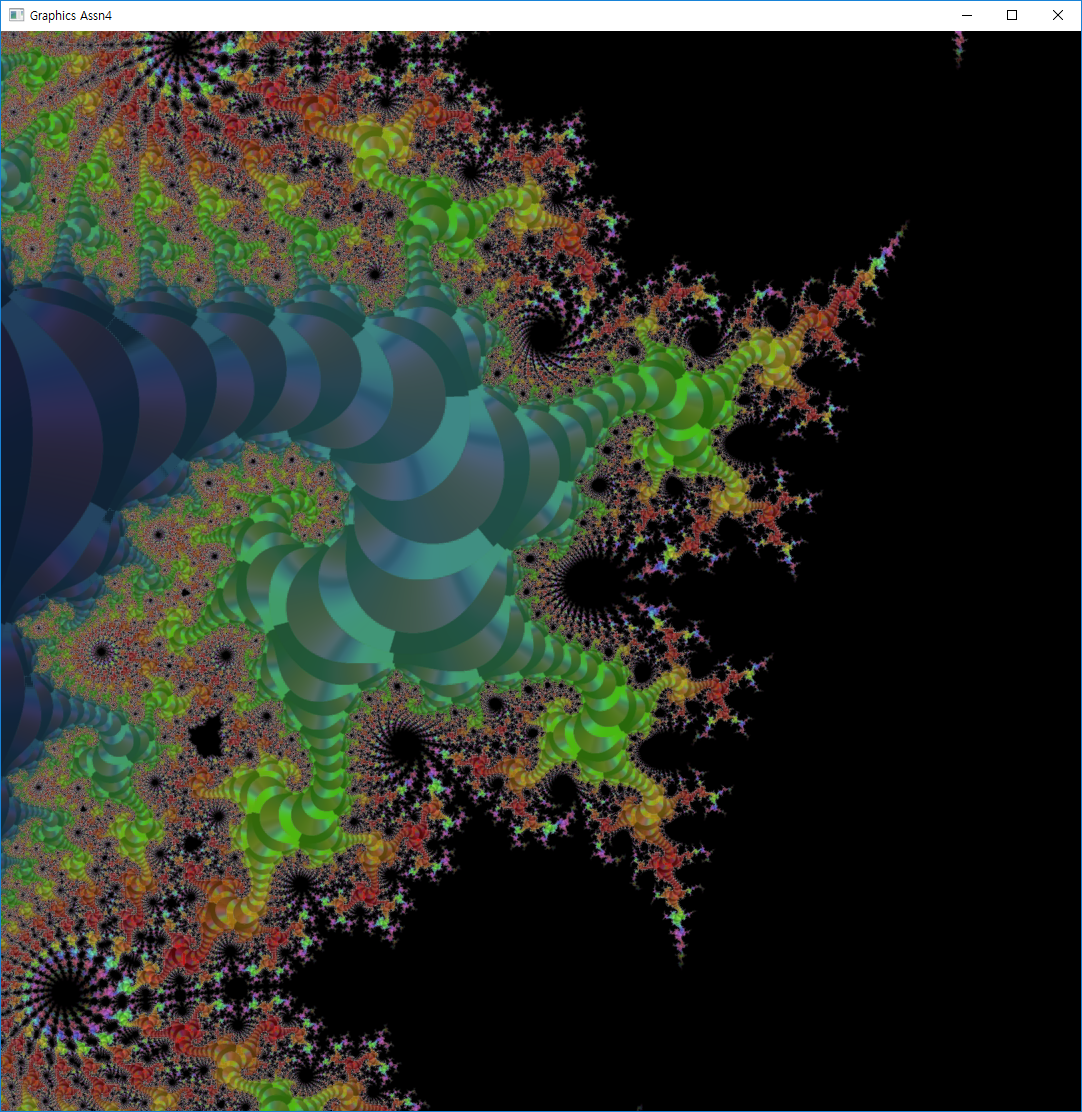
\includegraphics[scale=0.2]{anti.PNG}
}
\caption[1]{Antialiasing comparison}
\end{figure}

\section{Gallery}


We found that rendering quality has been improved but the rendering cost gets very expensive. (fps becomes $<20$)
One of our goal for this project is `real time', so we just discard the antialising.

\section{Discussion}
There are some issues in this project.
\begin{description}[style=nextline]
\item[hihi?]
byebye
\end{description}

\begin{thebibliography}{1}
\bibitem{c1}E. Angel and D. Shreiner, Interactive Computer Graphics: A Top-Down Approach with Shader-Based OpenGL, 6th ed., Addison-Wesley, 2011, p.487 Section 9.8 Recursive Methods and fractals
\bibitem{c2}Graham Sellers; Richard S. Wright, Jr.; Nicholas Hanemel, OpenGL SuperBible, 7th ed., Addison-Wesley, p.683 Rendering Julia Fractals
\bibitem{c3}Rickard Englund, Rendering Methods for 3D Fractals
\bibitem{c4}Fragmentarium,\url{http://syntopia.github.io/Fragmentarium/index.html}
\end{thebibliography}

\end{document}
